\subsubsection{Practical Applications}
\label{sub:dl_applications}

The previous chapter section covered recent progress in neural network research
on a theoretical level.
After gaining an understanding of modern architectures and training techniques,
this chapter will present practical applications of deep learning.
The upcoming subsections explain problems from multiple areas of computer
science, that can be approached using neural networks.
Namely, sections cover applications in Natural Language Processing (ch.~\ref{sub:dl_app_nlp}),
Computer Vision (ch.~\ref{sub:dl_app_cv}) and Reinforcement Learning (ch.~\ref{sub:dl_app_rl}).

\paragraph{Natural language processing (NLP)}
\label{sub:dl_app_nlp}

Section~\ref{sub:dl_architectures} introduced the problem of \textit{language modeling},
i.e., learning a probability distribution for words in a given sequence.
Convolutional and recurrent neural networks have been successfully applied to
this problem, in many cases improving previous state-of-the-art performance
on benchmark data sets.
Both network architectures are combined within complex models, so that these
so-called \textit{neural language models} are able to encode multiple
languages~\footcite{Kim2015}.
Another application of neural networks lies in the area of \textit{text classification},
i.e., assignment of a given text or document into predefined categories.
An example for this problem is classification of news articles into classes such
as sports, finance or politics.
This is an additional area in which deep learning shows increased performance
over previous approaches, mostly through the use of deep convolutional neural
networks~\footcite{Conneau2016}.
The most recently solved problem in natural language processing is \textit{machine
translation}, which aims to automate conversion of text between different
languages.
Complexity is here derived from the necessity of encoding the source language and
then decoding the learned representation into the target language.
Both model components, i.e., encoder and decoder, have shown to be efficiently
learnable with LSTMs (see ch.~\ref{sub:dl_architectures})~\footcite{Sutskever2014}.
The practical relevance of this research area is exemplified by contributions
from corporate research departments, e.g., \textit{Google}~\footcite{Wu2016}.

\paragraph{Computer vision}
\label{sub:dl_app_cv}

\begin{figure}[h]
  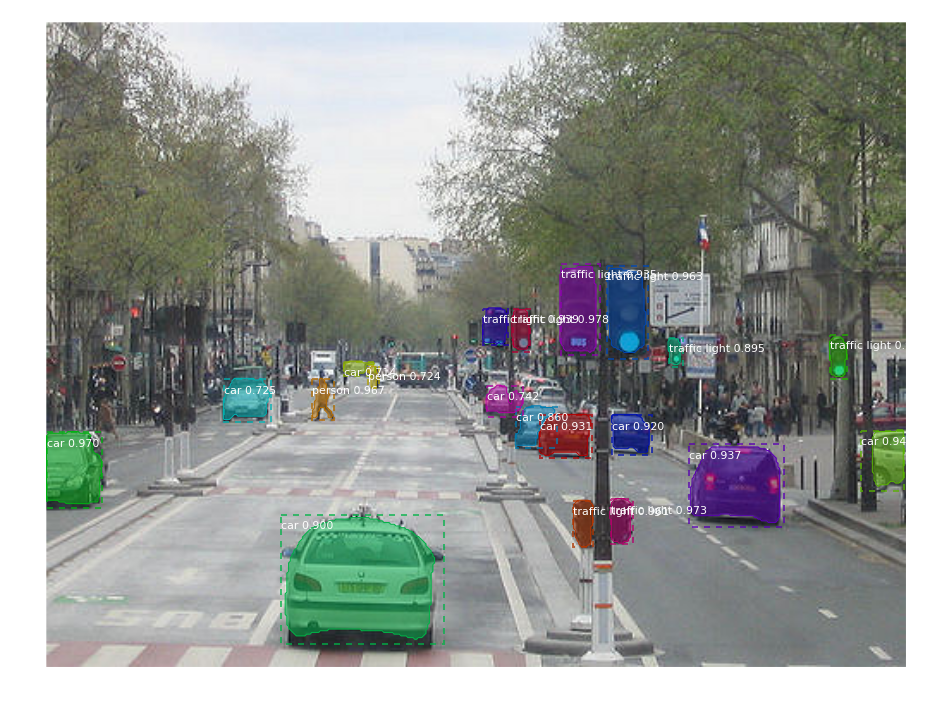
\includegraphics[height=10cm]{img/mask_rcnn}
  \caption[Object detection example]{Object detection example in street scenery~\footnote{\url{https://github.com/matterport/Mask_RCNN}}}
\label{fig:obj_detection}
\end{figure}

The area of computer vision mainly aims to process image and video data in
various ways.
Example problems that are solved using deep learning methods are presented in
the following.
As mentioned in previous chapters, \textit{image recognition} describes the
process of assigning images to categories.
Convolutional neural networks were designed to tackle problems like image
recognition by looking at individual sections of images using filters to
detect common features~\footcite{LeCun1998}.
Progress in deep learning allows training deeper models that contain more
convolutional layers and therefore can learn more complex features.
Thus, deep convolutional networks were able to push the state-of-the-art in image recognition~\footcite{Krizhevsky2012, He2016}.
\textit{Object detection} constitutes a related problem, whose goal is
to find all occasions of a predefined set of objects in an image.
Fig.~\ref{fig:obj_detection} shows an example image from a street scenery
with identified objects such as cars or traffic signals.
Deep learning models applied to object detection usually contain convolutional
layers to identify regions of interest in an image and map these to the
specified object classes~\footcite{Girshick2012, He2017}.
High-performance object detectors can then be used for even more advanced
tasks such as \textit{visual tracking}, i.e., following objects over several video
frames, or \textit{image captioning} which aims to describe images~\footcite{Bertinetto2016, Karpathy2017}.

\begin{figure}[h]
  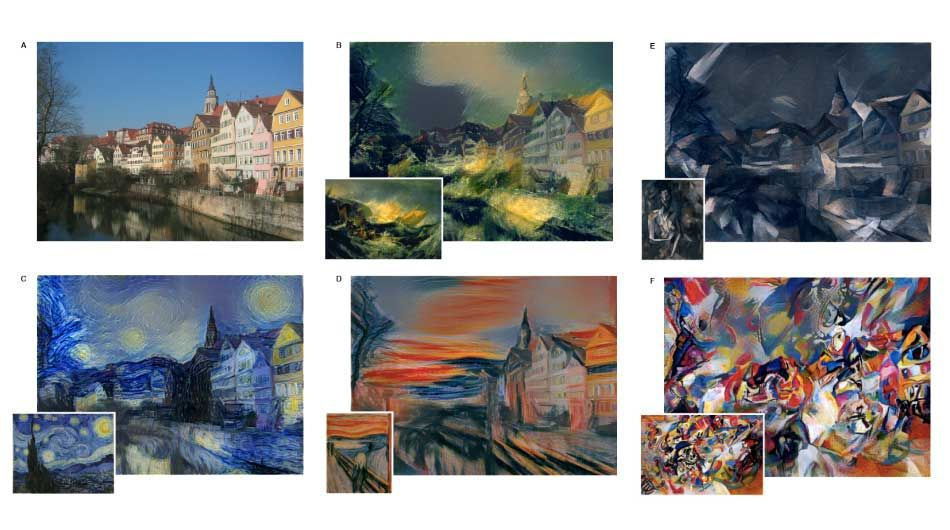
\includegraphics[height=9cm]{img/style_transfer.jpg}
  \caption[Style transfer example]{Style transfer example~\footcite{Gatys2015}}
\label{fig:style_transfer}
\end{figure}

Convolutional neural networks have also been used for generative tasks like
\textit{style transfer}.
Here, the goal is to apply styles of a source image, e.g., texture or colors,
to a target image.
An example is shown in Fig.~\ref{fig:style_transfer}, where a house scenery is
repainted in the style of various artists~\footcite{Gatys2015}.
Related tasks include image generation, where generative adversarial networks
show good performance~\footcite{Radford2015}.
Style transfer and image generation are also examples for unsupervised learning
problems, as introduced in ch.~\ref{sub:dl_terminology}, because there is
generally no labeled data for these tasks.

\paragraph{Reinforcement learning}
\label{sub:dl_app_rl}

Reinforcement learning constitutes another kind of experience for machine
learning algorithms.
In this setting, an agent continuously interacts with its environment and learns
from feedback in the form of rewards.
In order to estimate rewards for specific actions, the current state of the
given setting has to be evaluated.
Deep learning models have mostly been applied to evaluate settings that can
be displayed visually.
For example, this is the case for video games where each video frame represents an image.
Convolutional neural networks are used to detect patterns in the current
setting which are helpful for an agent and its decision about upcoming
actions.
Recently, researchers were able to train agents that perform better than human
professionals in several games, including simple \textit{Atari} video games
and more complex games like \textit{Go}~\footcite{Mnih2015, Silver2016}.

This chapter concludes the covered deep learning theory for this thesis.
The upcoming chapter explains basic concepts of social networks in general and
\textit{Twitter} more specifically, which are necessary for understanding
upcoming experiments.
